%&afbeeldingen
\documentclass[presentatie.tex]{subfiles}

\begin{document}

\section{Afbeeldingen}

\clearrecentlist

% \begin{frame}{Afbeeldingen}
% 	\begin{enumerate}
% 		\item \hll|\\includegraphics|
% 		\item Figure
% 		\item Nummering
% 		\item Naast elkaar (subfigure)
% 	\end{enumerate}
% \end{frame}

\addtorecentlist{\textbackslash includegraphics}

\begin{saveblock}{exinclgraph}
	\begin{highlightblock}[linewidth=0.95\textwidth,framexleftmargin=0.25em]
		Hier zie je een pingu~\"i~n:
		\includegraphics[height=2cm]{pinguin.jpg}
		Dit is een foto van het internet.
	\end{highlightblock}
\end{saveblock}

\newcommand\penExCode[2][2.5cm]{%
	%\adjustbox{max totalheight=2.5cm,set depth={\dimexpr 2.5cm-\height\relax},
	\adjustbox{%left=0.95\textwidth,bgcolor=gray!10!white,
		raise={-\height},set height=0cm,set depth=#1}{%
%		\parbox{\linewidth}{%
%			\hspace{-0.25em}\vrule width \dimexpr 0.95\textwidth+0.25em\relax depth 0px height 5.5px\par
%			\vspace{-\baselineskip}%
%			%
			\adjustbox{
				max totalheight=#1,
			%\adjustbox{max totalheight=2.5cm,min totalheight=2.5cm,raise={\depth},
				%bgcolor=red!5!white
			}{%
				\useblock{#2}%
				%\vfill%\leavevmode
			}%
%			\par
%			\hspace{-0.25em}\vrule width \dimexpr 0.95\textwidth+0.25em\relax depth 0px height 1px%
%		}
	}
	\par%\addvspace{0.0\baselineskip}%
	{\hspace{0.075\textwidth}\textcolor{red!30!white}{\rule{0.8\textwidth}{1px}}}\par
	\vspace{-\baselineskip}\vspace{0.3\baselineskip}%
	%%\par\addvspace{0.0\baselineskip}
}


\NewEnviron{penExResult}[1][3.5cm]{%
	%\adjustbox{raise={\depth},max height=4cm,set height=4cm,bgcolor=blue!5!white}{%
	%\adjustbox{max totalheight=3.5cm,set depth={\dimexpr 3.5cm-\height\relax},
	%\adjustbox{max totalheight=3.5cm,raise={\depth},set height=3.5cm,set depth=0pt,
	\adjustbox{max totalheight=#1,raise={-\height},set height=0cm,set depth=#1,
		%bgcolor=blue!5!white
	}{%
		\parbox{0.95\textwidth}{%
			\BODY
		}%
	}%
}

\begin{frame}{\adjustbox{raise=8px}{\hll|\\includegraphics|}}
	\vspace{-28px}
	\penExCode{exinclgraph}
	
%	\adjustbox{}{
%		bbb	
%	}
	
	\begin{penExResult}
		\only<2->{
			Hier zie je een pinguïn:
			\includegraphics[height=2cm]{assets/pinguin.jpg}
			Dit is een foto van het internet.
		}
	\end{penExResult}

\end{frame}

\begin{saveblock}{exinclgraph}
	\begin{highlightblock}[linewidth=0.95\textwidth,framexleftmargin=0.25em]
		Hier zie je een pingu~\"i~n:
		
		\includegraphics[height=2cm]{pinguin.jpg}
		
		Dit is een foto van het internet.
	\end{highlightblock}
\end{saveblock}

\addtorecentlist{als alinea}
\begin{frame}{\adjustbox{raise=8px}{\hll|\\includegraphics|}}
	\vspace{-28px}
	\penExCode{exinclgraph}
	
	\begin{penExResult}
		Hier zie je een pinguïn:
		
		\includegraphics[height=2cm]{assets/pinguin.jpg}
		
		Dit is een foto van het internet.
	\end{penExResult}
\end{frame}

\addtorecentlist{center}
\begin{saveblock}{exinclgraph}
	\begin{highlightblock}[linewidth=0.95\textwidth,framexleftmargin=0.25em]
		Hier zie je een pingu~\"i~n:
		\begin{center}
			\includegraphics[height=2cm]{pinguin.jpg}
		\end{center}
		Dit is een foto van het internet.
	\end{highlightblock}
\end{saveblock}

\begin{frame}{\adjustbox{raise=8px}{\hll|\\includegraphics|}}
	\vspace{-28px}
	\penExCode{exinclgraph}
	
	\begin{penExResult}
		Hier zie je een pinguïn:
		\begin{center}
			\includegraphics[height=2cm]{assets/pinguin.jpg}
		\end{center}
		Dit is een foto van het internet.
	\end{penExResult}
\end{frame}

\begin{saveblock}{exinclgraph}
	\begin{highlightblock}[linewidth=0.95\textwidth,framexleftmargin=0.25em]
		Een pingu~\"i~n zie je in \figref{fig:pinguin}.
		\begin{figure}[h]
			\centering
			\includegraphics[height=2cm]{pinguin.jpg}
			\caption{Een schattige pingu~\"i~n. Deze foto is van
				het internet.}\label{fig:pinguin}
		\end{figure}
	\end{highlightblock}
\end{saveblock}

\addtorecentlist{figure}
\begin{frame}{\adjustbox{raise=8px}{\hll|\\includegraphics|}}
	\vspace{-28px}
	\penExCode[3cm]{exinclgraph}
	
	\begin{penExResult}[3cm]
		Een pinguïn zie je in Figuur~\ref{fig:pinguin}.
		\begin{figure}[h]
			\centering
			\includegraphics[height=2cm]{assets/pinguin.jpg}
			\caption{Een schattige pinguïn. Deze foto is van het internet.}\label{fig:pinguin}
		\end{figure}
	\end{penExResult}
\end{frame}

\addtorecentlist{htbp}

\begin{frame}
	\frametitle{Figuurplaatsing}

	% Een figuur wordt ergens verderop geplaatst. Soms is het dus handig om een figuur
	% een paragraaf of twee the plaatsen voor de plek waar je hem gebruikt!
	
	\begin{itemize}
		\item h \textsc{(here)}: Figuur mag hier.
		\item t \textsc{(top)}: Figuur mag bovenaan een pagina.
		\item b \textsc{(bottom)}: Figuur mag onderaan een pagina.
		\item p \textsc{(page)}: Figuur mag op aparte pagina voor figuren.
		\item H \textsc{(here)}: Geen floating, altijd hier. (\hll|\\usepackage\{float\}|)
	\end{itemize}

	\medskip
	Te laat in output? Verplaats \hll|figure| naar voren in je bestand.
\end{frame}

\begin{saveblock}{subfigure}
	\begin{highlightblock}[linewidth=0.95\textwidth,framexleftmargin=0.25em]
		\begin{figure}[htbp]
			\centering
			\begin{subfigure}[b]{0.45\textwidth}
				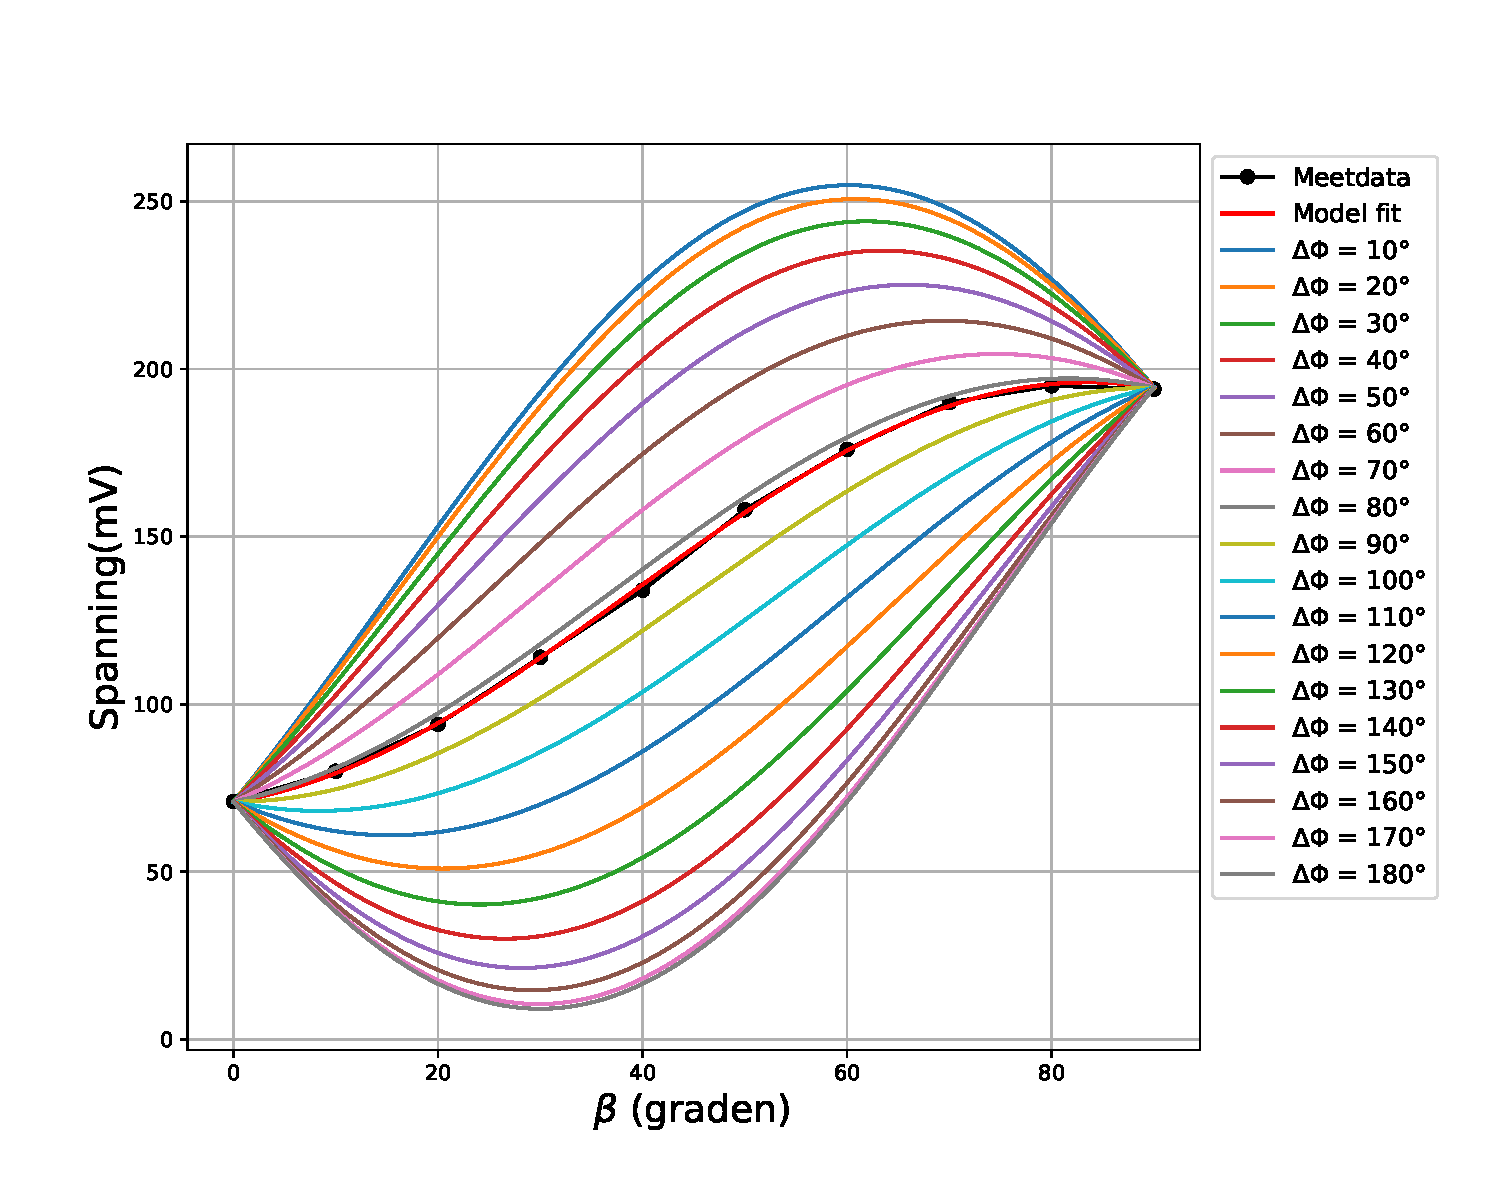
\includegraphics[width=\textwidth]{AA}
				\caption{BB}
				\label{fig:dphiExample}
			\end{subfigure}\qquad
			\begin{subfigure}[b]{0.45\textwidth}
				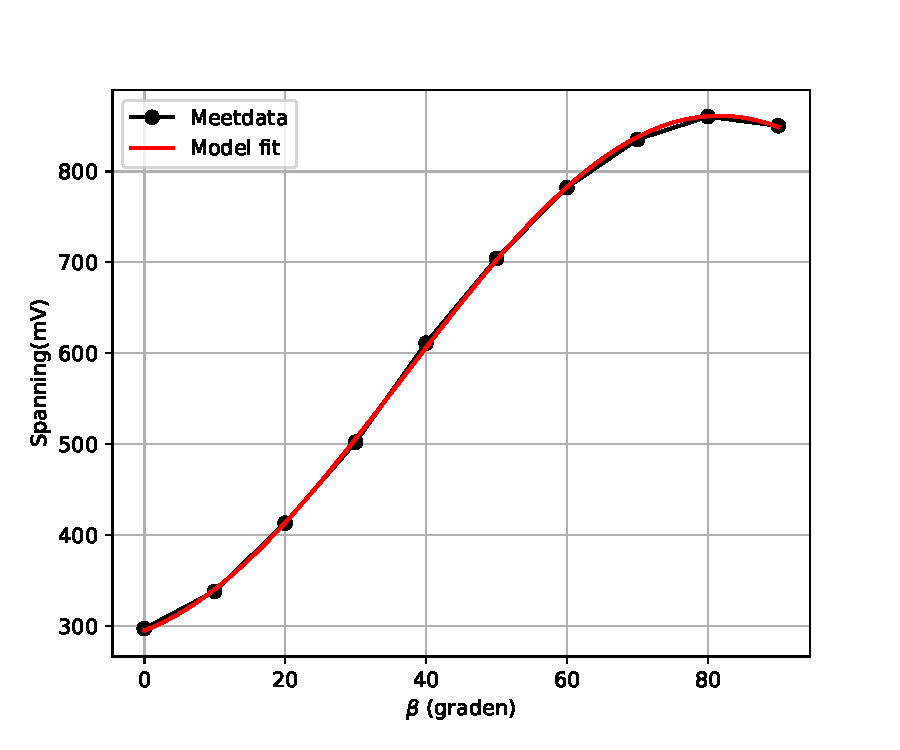
\includegraphics[width=\textwidth]{CC}
				\caption{CC}
				\label{fig:fitExample}
			\end{subfigure}
			\caption{Multiple images next to eachother!}
		\end{figure}
	\end{highlightblock}
\end{saveblock}

\addtorecentlist{subfigure}

\begin{frame}
	\frametitle{Subfigure \hll|(\\usepackage\{subcaption\})|}

	\useblock{subfigure}
\end{frame}

\begin{frame}
	\frametitle{Subfigure \hll|(\\usepackage\{subcaption\})|}

	\centering
	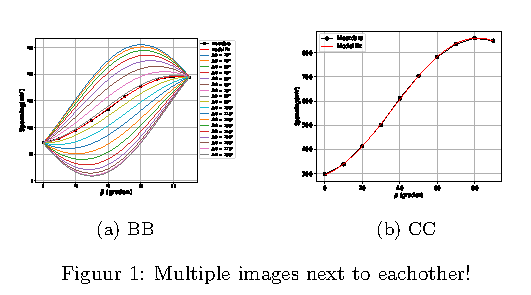
\includegraphics[width=\textwidth,height=0.8\textheight,keepaspectratio]{assets/4_Abeeldingen/outdir/subfigure}
\end{frame}

\end{document}
